\section{Experimental Methods} \label{sec:methods} 

It is not possible to induce a particular interaction in a particle collider: every physics process that $can$ occur from the collision of two protons at $13 TeV$ $will$ occur in the ATLAS detector. Thus, the process of studying rare Higgs interactions is not one of determining how to produce them in a laboratory setting, but of determining whether or not they are being produced in our detector at all. Because physics 'signal' processes are fundamentally indistinguishable from unwanted 'background' processes, ATLAS studies are statistical counting experiments which test the compatibility of the observed numbers of events with different detector signatures against the event counts that are predicted to occur under different physics hypotheses. 

Performing these experiments effectively in the data-rich environment of the LHC requires many clever statistical and computational tools, which vary from analysis to analysis. However, in all analyses, it is vitally important both to accurately model what the physics processes of interest may look like in the ATLAS detector and to translate observed detector signals into high-level physics objects. The Monte Carlo simulation method is used for the former, while the latter is performed by the variety of identification and reconstruction techniques detailed in this chapter.

\subsection{Monte Carlo} \label{sec:MC} 

The Monte Carlo simulation method is a way of modelling how a given physics process that may occur at the point of collision may translates into signatures in the ATLAS detector. For a given physics process, say, $gg \rightarrow t \bar{t} H$, we must model both the initial process (i.e., what is the likelihood two gluons will interact to make a $ttH$ event? What properties of the gluons make this more or less likely to occur? How will the top quarks and Higgs boson decay, and what might their decay products look like?), and the detector stage (how will the hadronic jets produced by decaying top quarks and the photons produced by a decaying Higgs look in the ATLAS detector?).

In order to make this problem computationally tractable, each stage is performed separately. In the first stage, the $generator$ stage, physics events for a given process are generated according to their cross-sections $\sigma$ (a measure of how likely they are to occur that is calculated using perturbation theory). A variety of different generator packages are used to produce events for different processes; common generator packages include PYTHIA \ref{Pythia}, HERWIG \ref{Herwig}, and aMCatNLO \ref{aMCNLO}. In many cases, intermediate decays are also performed by the generator software. Meanwhile, detector-level simulation is performed using the GEANT4 (GEometry ANd Tracking 4) package \ref{GEANT4}, which models the signatures of different particles produced in a collision as they pass through detector material.

Simulated events are then reconstructed in the same manner as real events. Because, unlike data events, Monte Carlo events include a "truth record" of what particles they contain, Monte Carlo simulations enable us to perform a number of useful tasks, including training machine learning algorithms to search for specific processes, model the relative contributions of various signal and background processes, and calculate various statistical and systematic uncertainties on our measurements \ref{1005.4568}.

\subsection{Reconstruction and Tagging} \label{sec:Reco} 

Objects produced in the ATLAS detector produce a wide variety of signatures, many of which can be difficult to distinguish from one another. For this reason, dedicated algorithms and criteria are employed to reconstruct and identify the particles used in ATLAS analyses. A sample illustration of the ATLAS detector showing typical shapes of a variety of physics objects is shown in Figure .

\begin{figure}
  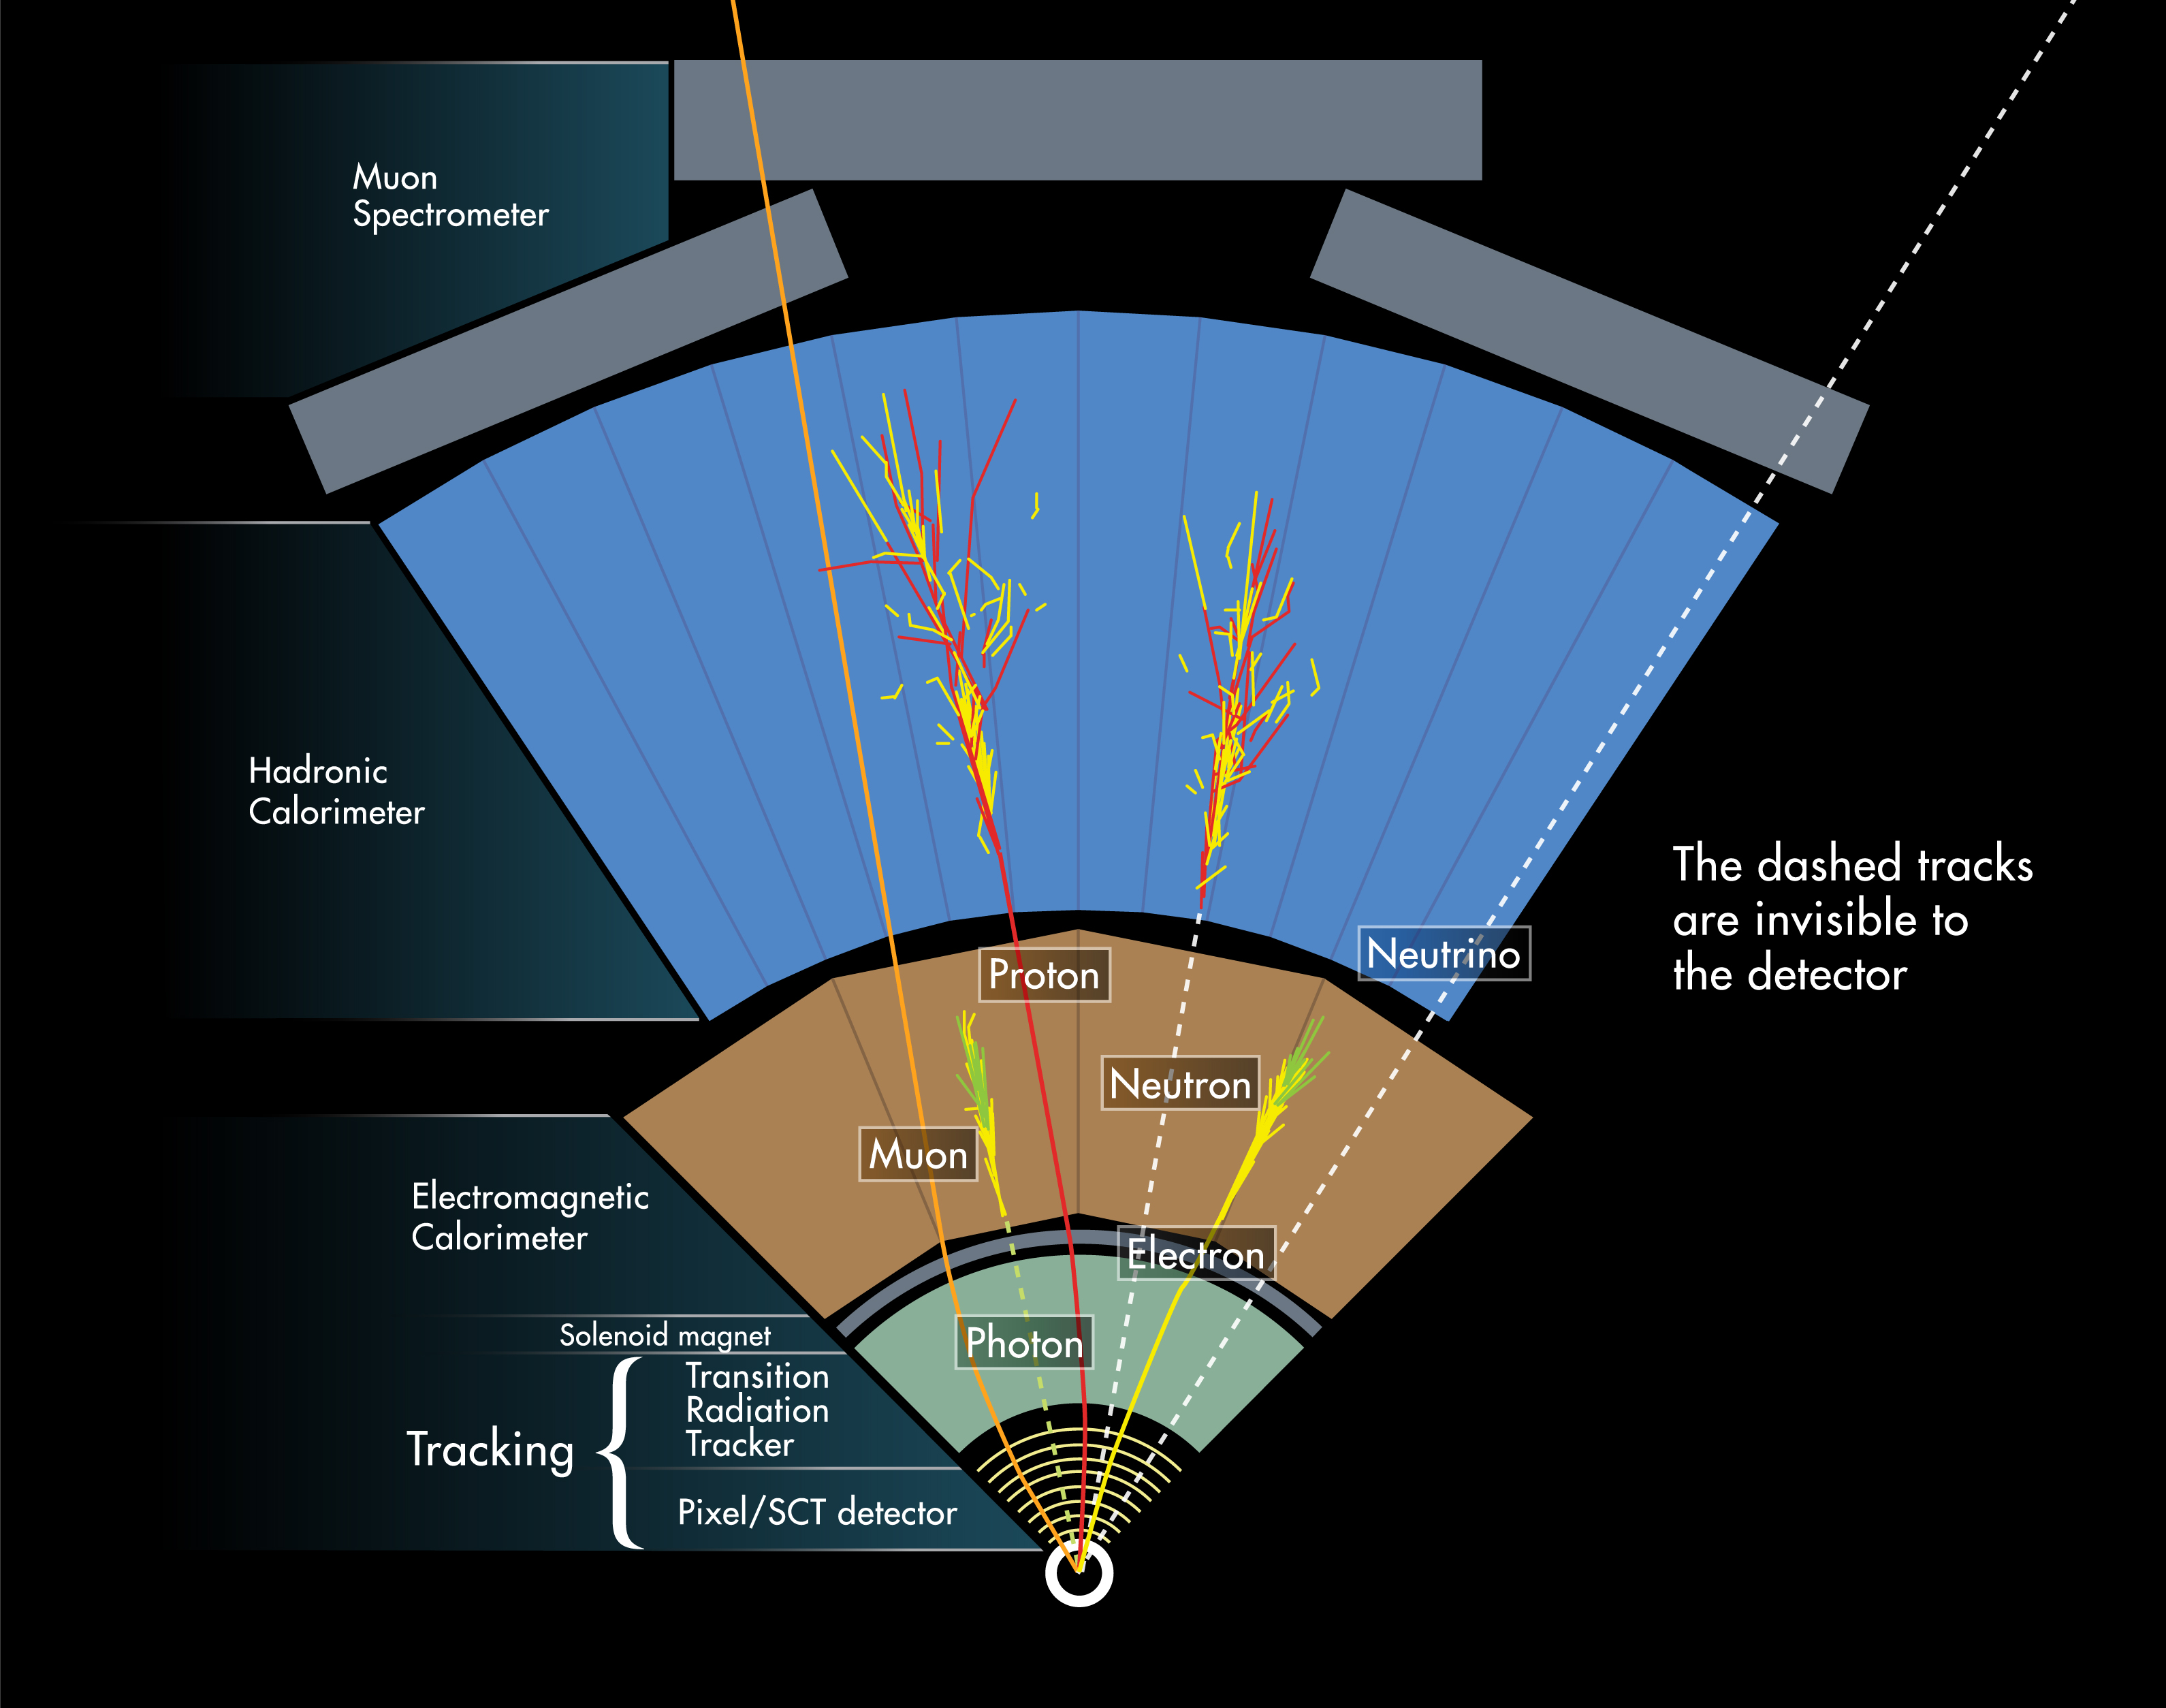
\includegraphics[width=\linewidth]{figures/methods_chapter/Sigs.jpg}
  \caption{Shapes and signatures of a variety of objects in the detector \ref{CERN-EX-1301009}}
  \label{fig:Signatures}
\end{figure}

\subsection{Tracks} \label{sec:Tracks} 

Track reconstruction is essential for identifying and measuring the properties of a wide variety of physics objects, including both muons and hadronic jets.

Initially, the "space points" (spatial coordinates) of potential particle hits are reconstructed using clusters of energy deposits in both the Pixel and SCT detectors. Track candidates are then identified combinatorially using this space-point information (with a minimum of three space-points per track candidate); these track candidates are then passed through an analytic weight-based "ambiguity solver" designed to weed out unphysical track candidates. To aid the ambiguity solver, a neural network is implemented in order to distinguish between isolated and merged clusters of energy deposits. After this, a neural network-based procedure is used to fit the identified tracks. \ref{cite:tracker}.

Fitted tracks from the Pixel detector and SCT can be extended into the TRT if nearby TRT hits are identified. In addition, tracks that are seeded by TRT hits can also be identified and reconstructed using an "outside-in" approach; this helps mitigate the potential loss of real tracks at the ambiguity-solver stage \ref{cite:NEWT}.

After tracks are identified and reconstructed, they are used to identify interaction vertices in the event. Each vertex candidate must contain at least two tracks, each with transverse momentum $p_{T} > 400$ MeV and $|\eta|<2.5$, at least nine hits in the Pixel or SCT detector for tracks with $|\eta|<1.65$ or at least eleven hits for tracks with $|\eta|>1.65$, at least one hit in the first two pixel layers (i.e., the IBL and the inner b-layer), no more than one shared module (i.e. one shared pixel hit or two shared SCT hits), no holes in the Pixel detector, and no more than one hole in the SCT. An iterative combinatorial procedure is then used to fit all compatible tracks to vertex candidates; the primary vertex (PV) representing the initial protom-proton collision is chosen as the vertex with the greatest $\Sigma p_{T}^{2}$ \ref{cite:VertexMeloni}.

However, we note that, for $H \rightarrow \gamma \gamma$ events, a potential lack of charged particles in the final state means that a different primary-vertexing method utilizing ECAL clusters must be considered. This is detailed at length in section \ref{sec:Electrons and Photons}.


\subsection{Clusters} \label{sec:Clusters} 

Photons, electrons and jets are reconstructed using topological clusters of hits ("topo-clusters") in the electromagnetic and hadronic calorimeters. Clusters are reconstructed using a "seed-and-collect" method, where cluster-initiating "seeds" are defined as calorimeter cells with an energy four times greater than the expected noise threshold for that cell  \ref{cite:CERN-EP-2019-145}, \ref{cite:CERN-PH-EP-2015-304}.

After the identification of seed cells, calorimeter cells neighboring the seed cell with recorded energy greater than twice their noise threshold are added to the proto-cluster. If proto-clusters contain more than two local maxima with energy greater than 500 GeV in a single cell, the proto-cluster is split into two in order to account for potential overlap. Initally, seed cells in these split clusters may reside only in the ECAL sampling layers EMB2, EMB3, EME2 and EME3, or the forward calorimeter module FCAL0, after this splitting, clusters are then iteratively split again, with maxima now allowed in the other HCAL and FCAL layers (The first layer of the ECAL is not used to seed topo-clusters in order to reduce the likelihood of producing clusters of noise). In the case of overlap between multiple clusters, cells are assigned to the two cluster candidates with the largest maxima.

\subsubsection{Electrons and Photons} \label{sec:Electrons} 

Electrons and photons are defined using tracks that are matched to topo-clusters in the ECAL. Topo-clusters compatible with EM showers are selected and used to define Regions of Interest; those Regions of Interest are then matched to tracks in the ID. Track candidates are extrapolated into the Regions of Interest using both the measured track momentum and the rescaled momentum measured in the relevant topo-cluster (the latter of which allows for accounting of radiative energy loss in the calorimeter). 

For a track to be considered matched to a topo-cluster, under either momentum-definition-extrapolation, it must fall within $|\Delta \eta| < 0.05$ of its relevant topo-cluster and satisfy $-0.10 < q \times (\phi_{track}-\phi_{cluster}) < 0.05$, where q is the charge of the incident particle. 

Topo-clusters matched to a single charged track are considered to be electron candidates, topo-clusters matched to two oppositely-charged tracks forming a vertex consistent with a photon are considered to be "converted" photon candidates (i.e., clusters resulting from a photon converting into and electron-positron pair in the ID), and topo-clusters matched to no tracks are considered to be "unconverted" photon candidates. In addition, single tracks that have no hits in the innermost layers of the ID are also considered as potential converted photon candidates\ref{cite:CERN-EP-2019-145}. 

Since the start of Run 2, combined topo-clusters called "superclusters" have been implemented in the EM clustering process in order to capture bremsstralung photons and other energy lost in the calorimeter \ref{cite:ATL-PHYS-PUB-2017-022}. For electrons, a supercluster seed must be a cluster with momentum $p_{T} > 1 GeV$ matched to a track with at least four hits, while for photons, a supercluster seed must be a cluster with momentum $p_{T} > 1.5 GeV$. Satellite clusters are then added to the seed to form a supercluster if they fall into a window $\Delta |\eta| \times \Delta\phi = 0.075 \times 0.125$ around the center of the seed cluster. For electrons, an additional satellite cluster search is performed, adding clusters that fall into the window $\Delta |\eta| \times \Delta\phi = 0.075 \times 0.125$ that are matched to the same track as the seed. For converted photons, the $\eta-\phi$ window is not used: all satellite clusters matched to one of the tracks of the converted photon vertex are added to the supercluster.

Following the identification of superclusters and tracks, energy calibration corrections are applied (determined using Monte Carlo simulation for photons and $Z \rightarrow ee$ decays for electrons)\ref{cite:EMcalib}, and the photon and electron candidate objects are passed to cluster-shape-based identification algorithms. For both electrons and photons, three identification working points are defined using cut-based multivariate discriminants based on the shower-shape variables.

For photons, the $loose$ ID threshhold is determined based on the following variables:
\begin{itemize}
  \item Acceptance: $|\eta|<2.37$, excluding the calorimeter crack at $1.37 <= |\eta|<1.52$  
  \item $R_{had}$: the ratio of transverse energy deposited in the HCAL to transverse energy deposited in the ECAL for clusters with $0.8 <= |\eta|<1.37$ 
  \item $R_{had1}$: the ratio of transverse energy deposited in the first layer of the HCAL to transverse energy deposited in the ECAL for clusters with $0.8 <= |\eta|<1.37$ 
  \item $R_{eta}$: the ratio of the energy deposited in the ECAL in a $3 \times 7$ rectangle in the $\eta \times \phi$ plane to the energy deposited in the ECAL in a $7 \times 7$ rectangle in the $\eta \times \phi$ plane, both centered on the calorimeter cell with the most deposited energy. 
   \item Lateral shower width $w_{eta2}$: $\sqrt{\frac{\sigma E_{i} \eta_{i}^{2}}{\sigma E_{i}}-{\frac{\sigma E_{i} \eta_{i}}{\sigma E_{i}}}^2}$ (where E is the energy and $\eta$ is the pseudorapidity of cell 'i', summed over all cells in a $3 \times 5$ rectangle centered around the most energetic calorimeter cell. 
\end{itemize}

The $medium$ photon ID threshold is determined based on both passage of the loose threshold and the variable $E_{ratio} = \frac{E_{1}-E_{2}}{E_{1}+E_{2}}$, where $E_{1}$ and $E_{2}$ are the leading and subleading energies deposited in calorimeter cells, respectively.

The $tight$ photon ID threshold is determined based on passage of the medium ID threshold and the following shape variables in the strip layer of the ECAL
\begin{itemize}
  \item Lateral Shower Width:$w_{s3} = \sqrt{\frac{\sigma E_{i}(i-i_{max})^{2}}{\sigma E_{i}}}$ (where E is the energy of a strip, '$i_{max}$' is the index of the highest-energy strip, and 'i' is the index of each strip with respect to $i_{max}$ calculated in a $3 \times 2 \eta-\phi$  rectangle centered around the strip with the maximum energy deposit
  \item Total Lateral Shower Width:$w_{s tot} = \sqrt{\frac{\sigma E_{i}(i-i_{max})^{2}}{\sigma E_{i}}}$ (where E is the energy of a strip, '$i_{max}$' is the index of the highest-energy strip, and 'i' is the index of each strip with respect to $i_{max}$ calculated in a $20 \times 2 \eta-\phi$  rectangle centered around the strip with the maximum energy deposit
  \item $\Delta E_{s}$: the difference between the second-largest strip energy and the minimum energy in the strips that lie between the largest- and second-largest strip energies
  \item $f_{1}$: The ratio of the energy in the first layer to the energy in the whole EM cluster.
  \item $f_{side}$: the total energy outside the three central strips but within seven strips, divided by the energy of the three central strips 
\end{itemize}

Each working-point threshold varies in bins of $\eta$. For loose and medium working points, converted and unconverted photons are not treated differently, but for tight working points, they are determined separately. \ref{cite:gammaID CERN-EP-2018-216}

For electrons, the identification process proceeds similarly: working-points are defined using shower-shape variables $f_{1}, E_{ratio}, w_{s tot}, R_{eta}, w_{eta2}, f_{3}, R_{had}, and R_{had1},$ as well as $R_{phi}$ (the ratio of the energy deposited in the ECAL in a $3 \times 3$ rectangle in the $\eta \times \phi$ plane to the energy deposited in the ECAL in a $3 \times 7$ rectangle in the $\eta \times \phi$ plane, both centered on the calorimeter cell with the most deposited energy). Electron ID working-points also include the following track variables:
\begin{itemize}
\item $n_{Blayer}$: Number of hits in the B-layer
\item $n_{Pixel}$: Number of hits in the Pixel
\item $n_{Si}$: Number of hits in the silicon detectors (ID and SCT)
\item $d_{0}$: the transverse impact parameter relative to the beamline
\item $|d_{0} / \sigma(d_{0})|$: the impact parameter significance relative to its uncertainty
\item $\Delta(p)/p = (p-p_{last})/p$: the momentum difference between the track perigee and its endpoint, divided by the momentum at perigee
\item $eProbabilityHT$: the electron probability based on TRT radiation
\item $\Delta \eta_{1}$: the difference in pseudorapidity between the cluster position in the first layer and the matched track
\item $q \times (\phi_{track}-\phi_{cluster})$: where $\phi_{track}$ is the momentum-rescaled track extrapolated from the perigee and $\phi_{cluster}$ is the cluster position in the second ECAL layer.
\item $E/p$: ratio of the cluster energy to the track momentum (used for $E_{T} > 150 GeV$ only) 
\end{itemize}

However, the photon identification is a cut-based process, while the electron identification process relies on a likelihood-based discriminant. For the analyses discussed in subsequent chapters, we utilize the $Medium$ electron working point, with an efficiency of approximately 88$\%$ \ref{cite:elID-CERN-EP-2018-273}. Electrons are also required to satisfy $p_{T} > 10 GeV, |\eta| < 2.47$ (excluding the calorimeter crack at ($1.37<|\eta|<1.52$), have track impact parameter significance $|d_{0} / \sigma(d_{0})| < 5$, and satisfy $z_{0} \times sin(\theta) < 0.5 mm$ with respect to the primary vertex \ref{ATL-COM-PHYS-2020-378}.

To aid in modelling, additional photon ID working points are created. These "LoosePrimeN" working points involve photons that pass the 'loose' identification criteria, but fail one or more of N 'tight' identification criteria. The analyses discussed in this dissertation use the LoosePrime4 working point, which is defined as photons passing the Loose identification but failing one or more of the $w_{s3}, f_{side}, \Delta E_{s}$, and $E_{ratio}$ criteria \ref{ANA-EGAM-2018-01}.

To distinguish between photons originating from the hard scatter (i.e., the process of interest in an event) and photons radiated off of other final-state objects, we consider the relative isolation of identified photons. Photons near large amounts of calorimeter activity are likely to be radiative photons ('non-prompt') radiated from final-state particles after the hard-scatter event, while photons that are isolated are more likely to originate from the hard-scatter.

Two types of isolation variables are considered: calorimetric and track-based.

The calorimetric isolation variable employed in the analyses discussed here is $E_{T}^{coneXX} = E_{T,raw}^{isolXX} -E_{T}^{core} - C$, where $E_{T,raw}^{isolXX}$ is the total calorimeter energy in a cone of $\Delta R = XX/100 $ around the electron or photon of interest, $E_{T}^{core}$ is the total calorimeter energy in a $5 \times 7$ rectangle in $\Delta \eta \times \Delta \phi$ around the barycenter of the electron or photon of interest, and C is a correction for pileup and leakage.

The photon track isolation variable employed in the analyses discussed here is $p_{T}^{cone20} = p_{T}^{cone} - p_{T}^{core}$, where $p_{T}^{cone}$ is the total track momentum of all tracks with $p_{T} > 1GeV$ in a cone of $\Delta R = 0.2$ around the photon of interest and $p_{T}^{core}$ is the total track momentum of all tracks with $p_{T} > 1GeV$ matched to the photon candidate. In addition to satifying $p_{T} > 1GeV$, all tracks considered for this metric must also fall within $z= 3mm$ of the diphoton vertex and have $|\eta|<2.5$.

The electron track isolation variable considered is $p_{T}^{varcone20}$, identical to $p_{T}^{cone20}$ except for the fact that, rather than consider a constant-radius cone of $\Delta R = 0.2$, we consider a cone of radius $\Delta R = max(\frac{10}{p_{T}[GeV]}, 0.2)$ \ref{cite:CERN-EP-2019-145}.

Unlike in Run 1, photon isolation cut thresholds are defined as a function of photon energy rather than being fixed. The isolation thresholds used are $FixedCutLoose$ ($E_{T}^{cone20}< 0.065 E_{T}^{\gamma}$ and $p_{T}^{cone20} < 0.05 E_{T}^{\gamma}$) and $FixedCutTight$ ($E_{T}^{cone40}< 0.022 E_{T}^{\gamma} + 2.45 GeV$ and $p_{T}^{cone20} < 0.05 E_{T}^{\gamma}$) for photons and $FCLoose$ ($E_{T}^{cone20}< 0.2 p_{T}$ and $p_{T}^{cone20} < 0.15 p_{T}$) for electrons \ref{cite:ATL-COM-PHYS-2020-378}.

In analyses discussed in this dissertation, the diphoton vertex originating from the Higgs decay is often not the hardest vertex. This is because, in processes such as gluon-gluon fusion ($ggF$), many events contain a low final-state track multiplicity \ref{1408.7084}. The diphoton vertex is therefore identified using a Neural Network, trained on variables including the $photon pointing$ (that is, the vertex position in $z$ most compatible with the shower-shapes observed in the ECAL), the $\Delta \phi$ between the vector sum of the track momenta and the diphoton system (as determined by the ECAL), and the scalar momentum sums $p_{T}$ and $p_{T}^2$ for the tracks in each diphoton vertex candidate \ref{HGAMSTXSINT}. Photon energies and pseudorapidities are corrected to reflect this new vertexing procedure.

The efficiency of the Neural Network diphoton vertex compared to the hardest vertex for a number of targeted physics processes ("STXS bins") for the full Run-2 Couplings analysis is shown in Figure .

\begin{figure}
  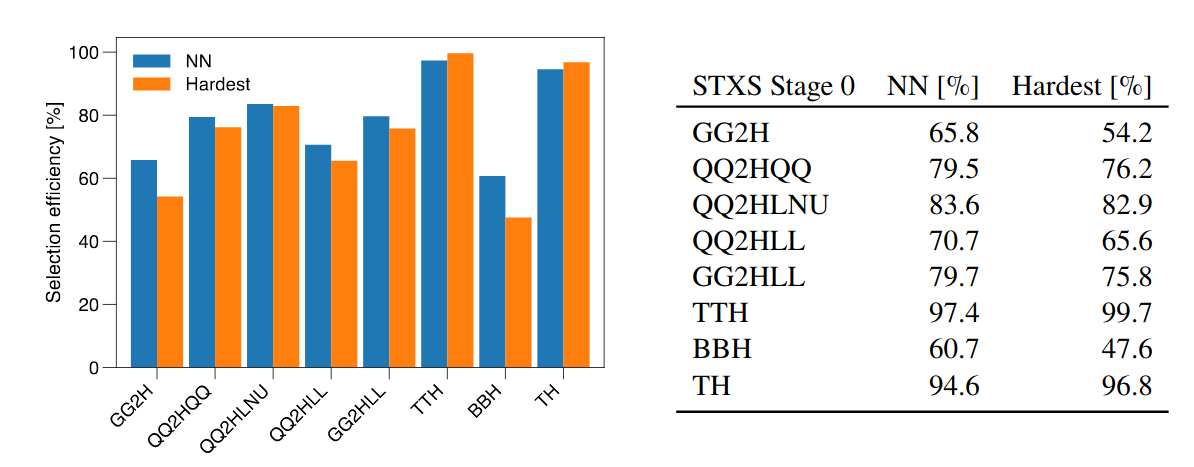
\includegraphics[width=\linewidth]{figures/methods_chapter/Vertexing.png}
  \caption{Shapes and signatures of a variety of objects in the detector \ref{ATL-COM-PHYS-2020-378}}
  \label{fig:Vertexing}
\end{figure}

\subsubsection{Jets} \label{sec:Jets} 

Hadronic jets are identified from topo-clusters using the $anti-k_{t}$ algorithm. Clustering algorithms iteratively follow the following procedure: for each topo-cluster $i$, calculate the distance between both the topo-cluster and every other topo-cluster $j$ and between the topo-cluster and the beam $B$: 

\begin{equation} 
d_{i,j} = min(p_{T,i}^{2k}, p_{T,j}^{2k})\frac{((y_{i}-y_{j})^{2}-(\phi_{i}-\phi_{j})^{2})}{R^2}
d_{i,B} = p_{T,i}^{2k}
\end{equation} 

Where $y_{i}$ is the rapidity of particle $i$, defined as $y=\frac{1}{2} ln(\frac{ E + p_{L}}{ E - p_{L}})$ (where $p_{L}$ is the particle's momentum in the beam direction), $R = 0.4$ (the jet radius), and k is some constant. For the anti-$k_{t}$ algorithm, $k = -1$; other common clustering algorithms use $k=1$ ($k_{t}$) or $k=0$ (Cambridge-Aachen). 

After calculating these metrics, combine the two cluster objects that are the smallest distance apart and re-calculate the distance metrics for the combined object. If a cluster object is closer to the beam than to another object, it is considered a jet and is removed from the list of objects for potential combination.

The algorithm is both infrared safe, meaning that very-low-$p_{T}$ objects do not appreciably impact the jet-finding algorithm results, and collinear safe, meaning that splitting one high-$p_{T}$ object into two collinear ones does not impact the results. Compared to other jet-finding algorithms, the anti-$k_{T}$ algorithm is more robust to the effects of low-energy radiation \ref{antikt}.

For the Run-2 Couplings analysis detailed in section \ref{sec}, the ParticleFlow algorithm detailed in ref \ref{PFlow} is implemented. This helps to provide clearer pictures of the individual constituents of a jet. The ParticleFlow algorithm is an intermediate step in jet reconstruction, which subtracts off energy deposits not associated with the primary vertex and replaces energy deposits that are associated with the primary vertex with the momenta of the relevant tracks. This is done using the modified diphoton vertex discussed previously.

The collection of jets is "cleaned" to remove jets that have signatures consistent with calorimeter noise, and jets that do not satisfy $|y| < 4.4$ and $p_{T} > 25 GeV$ are rejected as well. 

A Jet Vertex Tagger (JVT) multivariate discriminant is also used to reject pileup jets. This utilizes variables such as Jet Vertex Fraction (the $p_{T}$ in a given jet that is track-associated to the primary vertex divided by the $p_{T}$ in a given jet that is track-associated to all vertices) and $R_{pT}$ (the fraction of the $p_{T}$ in a given jet that is track-associated to the primary vertex divided by the total jet $p_{T}$). Different JVT thresholds are used for PFlow Jets and the standard "EMTopo" jets that do not use the ParticleFlow algorithm \ref{cite:JVT}.

\subsubsection{b-jets} \label{sec:b-jets} 

While in general it is very difficult to identify thetype of particle that seeded a hadronic jet, jets originating from hadrons containing bottom quarks are often identifiable with some degree of accuracy. This is due to their long lifetimes compared to other hadrons, meaning that they will travel a short distance in the inner detector (~$450 \mu m$) before hadronizing into jets. 

For EMTopo jets, the Boosted Decision Tree-based Mv2c10 algorithm is used, while for ParticleFlow jets, the Neural Network-based DL1r algorithm is used. The Mv2c10 algorithm is based on a Boosted Decision Tree trained on variables such as impact parameter significance, the presence ad properties of a secondary vertex, and jet kinematic variables such as $p_{T}$ and $\eta$ \ref{cite:CERN-EP-2018-047, CERN-PH-EP-2015-216}; the DL1r algorithm is based on a Deep Neural Network \ref{cite:ATL-PHYS-PUB-2017-013} trained on the same input variables as the Mv2c10 tagger, with additional vertex variables included to allow for charm-quark jet discrimination. The DL1r tagger also features a recurrent neural network trained to take advantage of correlations between track impact parameters in discrimination. The Mv2c10 tagger has an efficiency of approximately 77$\%$, while the DL1r has an efficiency of approximately 70$\%$.  

\subsubsection{Muons} \label{sec:Muons} 

Muons are reconstructed using tracks from either the muon spectrometer and inner detector or the muon spectrometer only.

In the muon spectrometer, segments of hits along the bending plane in the MDT chambers are identified using a Hough transform \ref{Hough}, an image-processing technique from the field of edge-detection that maps observed line segments into a polar-coordinate feature space. The coordinate orthogonal to the bending plane is found using TGC and RPC hits, while segments in the CSC detectors are reconstructed using a separate combinatorial algorithm. Muon tracks are then reconstructed from the segments using a $\chi^{2}$ algorithm- a track must contain at least two segments, except in the barrel-endcap transition region, where one segment is sufficient to build a track. 

Tracks are used to define four types of muons: Combined Muons, for which a track is fitted using both the Inner Detector and Muon Spectrometer, Segment-Tagged, for which a track in the ID is matched to a segment (but not a full track) in the Muon Spectrometer, Calorimeter-Tagged for which a track in the ID is matched to a calorimeter deposit compatible with a muon, and Extrapolated Muons, reconstructed using segments in the Muon Spectrometer that are not associated with any ID tracks but are compatible with the primary vertex. For all muons using the ID, criteria on the number of hits in each ID subsystem are employed to ensure track quality.

Muons must also pass identification criteria to distinguish them from potential fake muons (usually pions or kaons). Three main criteria are used:

\begin{itemize}
\item The charge-to-momentum ratio significance, defined as the absolute value of the difference between the ratio of the charge and momentum of the muons measured in the ID and MS divided by the sum in quadrature of thecorresponding uncertainties
\item $\rho'$, defined as the absolute value of the difference between the transverse momentum measurements in the ID and MS divided by the $p_{T}$ of the combined track
\item the normalized $\chi^{2}$ of the combined track fit
\end{itemize}

The analyses detailed in this thesis use the Medium identification working point, which allows only Combined and Extrapolated muons. Medium Combined Muons require at least 3 hits in at least two MDT layers, except for tracks in the $|\eta| <0.1$ region, where tracks containing at least one MDT layer but no more than one MDT hole layer are allowed. Medium Extrapolated muons require at least three MDT or CSC hits, and are only used in the region $2.5 < |\eta| < 2.7$. Additionally, the q/p significance is required to be less than 7 \ref{CERN-EP-2016-033}. 

Like other objects, we require isolated muons. Muon isolation variables are defined identically to those of electrons for the ttH-CP analysis, while for the Couplings analysis, the ParticleFlow algorithm is used to augment the isolation procedure with a new isolation variable called $neflowiso$, corresponding to the energy deposited in neutral reconstructed ParticleFlow objects rather than raw calorimeter clusters \ref{ATL-COM-PHYS-2019-177}.

For the standard isolation, we use the $FixedCutLoose$ working point, corresponding to $E_{T}^{cone20}<0.30 \times p_{T}^{\mu}$ and $p_{T}^{varcone30}<0.15 \times p_{T}^{\mu}$. For the ParticleFlow isolation, we use $(ptvarcone30+ 0.4\times neflowisol20) <0.16 \times p_{T}$ for muons with $p_{T} < 50GeV$ and $(ptvarcone20+ 0.4\times neflowisol20) < 0.16 \times p_{T}$ for muons with $p_{T} > 50GeV$.

Additionally, muons are required to satisfy $p_{T} > 10 GeV, |\eta| < 2.7$, have track impact parameter significance $|d_{0} / \sigma(d_{0})| < 3$, and satisfy $z_{0} \times sin(\theta) < 0.5 mm$ with respect to the primary vertex \ref{ATL-COM-PHYS-2020-378}. Muon momentum and energy scale and resolution calibrations are determined using $J/\psi \rightarrow \mu \mu$ and $Z \rightarrow \mu \mu$ decays \ref{cite:muCalib}. A charge-dependent sagitta bias calibration is also applied to correct for a slight observed misalignment of the muon system and inner detector.

\subsubsection{Overlap Removal} \label{sec:Overlap}

An overlap removal procedure is employed to avoid double-counting objects. It proceeds in the following order:

\begin{itemize}
\item Remove electrons within $\Delta R=0.4$ of any photon
\item Remove muons within $\Delta R=0.4$ of any photon
\item Remove jets within $\Delta R=0.4$ of any photon
\item Remove jets within $\Delta R=0.2$ of any electron
\item Remove electrons within $\Delta R=0.4$ of any jet
\item Remove muons within $\Delta R=0.4$ of any jet
\end{itemize}

\subsubsection{MET} \label{sec:MET}

The initial momentum of protons approaching the collision point is almost entirely in the beam direction, that is, there is no appreciable momentum component in the transverse direction. Thus, by conservation of momentum, we expect that, when we sum the momenta of all particles produced in the event, we should not see an appreciable momentum excess in the transverse direction. However, often such an excess does occur, indicating the presence of undetected particles that have caused the visible transverse momentum imbalance. Missing Transverse Energy, or MET, is something of a misnomer, as it is missing $momentum$, not energy, but it is one of the most valuable tools for studying rarely-interacting particles such as neutrinos in the ATLAS detector.

The MET is defined as the negative vector sum of the transverse  momenta of all objects associated with the diphoton vertex, including electrons, photons, muons, jets, and any additional low-$p_{T}$ tracks. For the purpose of MET reconstruction in $H \rightarrow \gamma \gamma$ events, $\tau$ leptons are treated as jets; this is allowable because they occur rarely in the parameter spaces studied and decay dominantly to hadrons \ref{cite:CERN-EP-2017-274}.

\subsubsection{taus} \label{sec:taus}
We note that, though many physics analyses use $\tau$ leptons, they are not considered in any of the event signatures discussed in this thesis, so we refrain from discussing their reconstruction at length. However, we note that tau leptons can decay both hadronically and leptonically; as a result of this, their reconstruction depends on the reconstruction of electrons, muons, and jets.
